\documentclass[letterpaper]{article}
\usepackage[multiple]{footmisc}
\usepackage{natbib,alifeconf}  %% The order is important
\usepackage{placeins}
\usepackage{hyperref}

\usepackage{graphicx,environ}

\newsavebox{\figsavebox}% Box to capture figure content

\newif\ifhidefigures % Conditional to hide figures or keep them in the document

\NewEnviron{conditionalfigure}[1][ht]{%
  \ifhidefigures
    % Hide this figure
    \let\oldlabel\label
    \renewcommand{\label}[1]{\gdef\labelname{##1}}% Store label name
    \renewcommand{\caption}[1]{##1}% Make \caption just print its argument
    \begin{lrbox}{\figsavebox}
      \BODY % Capture enture figure body
    \end{lrbox}
    \refstepcounter{figure}\oldlabel{\labelname}% Step counter with reference and mark with label
  \else
    % Traditional figure environment
    \begin{figure}[#1]
      \BODY
    \end{figure}
  \fi
}

% *****************
%  Requirements:
% *****************
%
% - All pages sized consistently at 8.5 x 11 inches (US letter size).
% - PDF length <= 8 pages for full papers, <=2 pages for extended
%    abstracts (not including citations).
% - Abstract length <= 250 words.
% - No visible crop marks.
% - Images at no greater than 300 dpi, scaled at 100%.
% - Embedded open type fonts only.
% - All layers flattened.
% - No attachments.
% - All desired links active in the files.

% Note that the PDF file must not exceed 5 MB if it is to be indexed
% by Google Scholar. Additional information about Google Scholar
% can be found here:
% http://www.google.com/intl/en/scholar/inclusion.html.


% If your system does not generate letter format documents by default,
% you can use the following workflow:
% latex example
% bibtex example
% latex example ; latex example
% dvips -o example.ps -t letterSize example.dvi
% ps2pdf example.ps example.pdf


% For pdflatex users:
% The alifeconf style file loads the "graphicx" package, and
% this may lead some users of pdflatex to experience problems.
% These can be fixed by editing the alifeconf.sty file to specify:
% \usepackage[pdftex]{graphicx}
%   instead of
% \usepackage{graphicx}.
% The PDF output generated by pdflatex should match the required
% specifications and obviously the dvips and ps2pdf steps become
% unnecessary.


% Note:  Some laser printers have a serious problem printing TeX
% output. The use of ps type I fonts should avoid this problem.


\title{MODES Analysis of Prediction Games}


%%do not add authors names, review process will be double blind 
\author {Thomas Willkens \and Jordan Pollack\\
\mbox{} \\
%       \author {Author 1$^{1}$ , Author 2$^{2}$ ... \and Author n$^{n}$\\
%       \mbox{} \\
Dynamical and Evolutionary Machine Organization Lab \\ 
Brandeis University, Waltham, MA, USA \\
twillkens@brandeis.edu, pollack@brandeis.edu
}

\begin{document}
\hidefigurestrue % Remove conditional figures from document
\maketitle





\begin{abstract}
% Abstract length should not exceed 250 words
Much activity in the field of artificial life has been concerned with the search for appropriate and effective methods of quantifying \textit{open-ended} behavior in evolutionary systems. The MODES Toolbox is a recent addition that employs a persistence filter over evolutionary lineages to focus attention only on those genotypes that are most adaptive. The Toolbox provides a useful and intuitive set of metrics in terms of change, novelty, complexity, and ecology. One domain thought to exhibit open-ended dynamics, the linguistic prediction game, is a ripe candidate for deeper statistical analysis. We apply the MODES Toolbox on this domain, lending support to prior hypotheses regarding evolutionary stable states while also suggesting that, in at least one case, the observed complexity growth is largely nonadaptive. 
\end{abstract}

\section{Introduction}

The emerging field of \textit{open-endedness} seeks to understand the properties of systems that never settle into an equilibrium state, with the hope of channeling this knowledge into richer scientific explanations and practical applications \citep{OEE4-2021, stanley2019,stepney2021,soros2018,taylor2019}. The \textit{MODES Toolbox} (Measurements of Open-Ended Dynamics in Evolving Systems) \citep{dolson2019} aims to provide a set of domain-independent metrics for assessing open-ended behavior in evolutionary systems. Its primary tool is the \textit{persistence filter}, a method informed by \textit{coalescence theory} for pruning maladaptive and neutral clades from the dataset so that closer attention can be paid to long-lasting lineages \citep{Fu1999CoalescingIT}. Intuitive and simple metrics such as novelty, change, and ecology may be applied to these individuals, provided the genotype is pruned of neutral or harmful sites. 

We apply this toolbox to the \textit{linguistic prediction game} \citep{moran2019}, a coevolutionary domain with some configurations thought to exhibit open-ended \textit{complexity growth}, to better grasp its statistical properties from a different perspective. Prior literature suggests the relevancy of competition, cooperation, and coevolution to the phenomenon of complexity growth \citep{zaman2014,Soros2014IdentifyingNC,dolson2021}, and so a thorough appraisal of this relatively simple domain could prove generally useful. An \textit{adaptive pruning} heuristic is proposed to remove nonadaptive sites in genotypes represented by \textit{deterministic finite state machines} (DFSMs). 

Prior hypotheses regarding cycling behavior in competitive ecosystems are supported by observations of decreasing rates of novelty. We also discover evidence that--for at least one ecosystem--the prior complexity metric obtained through \textit{Hopcroft minimization} \citep{Hopcroft1971AnNL} of the genotypes insufficiently captures the dynamics of the overall system. Namely, we find that the apparently unbounded complexity growth seen in the \textit{Three-Species Mixed} ecosystem appears largely nonadaptive. 

\section{Background}
\subsection{The Linguistic Prediction Game}
The linguistic prediction game is a coevolutionary domain proposed in \cite{moran2019} for the purpose of exploring the dynamics of evolutionary complexity growth. Members of different populations are matched in pairwise fashion in different classes of interactions. In the game, each player simultaneously emits a bit; if the game is \textit{cooperative}, then players share the same goal: either to match (or mismatch) the bit provided by the other. In a \textit{competitive} interaction, however, only one player is rewarded for matching (or mismatching) bits. Neither player is aware of the nature of their relationship upon starting the game, and their decisions must be made based solely on the patterns of bits produced.

\begin{figure}[t]
    \begin{center}
        \includegraphics[width=2.5in]{img/ecos.png}
        \caption{Ecosystems considered in this work. A line with no arrow indicates interaction between control groups. A line with an arrow indicates a competitive interaction in which the species pointed to seeks to match bits while the other seeks to mismatch. A line with two arrows indicates a cooperative interaction wherein both seek to match; a dotted line indicates a cooperative interaction where both seek to mismatch.}
        \label{ecosystems}
    \end{center}
\end{figure}

An \textit{ecosystem} is a coevolutionary configuration involving two or more populations and the arrangement of interactions between them. In the \textit{Two-Species Cooperative} (Coop) variety, both seek either to match or mismatch bits. The \textit{Two-Species Competitive} (Comp) ecosystem involves two populations: one whose members seek to match bits, and another whose members seek to mismatch; the \textit{Three-Species Competitive} (3-Comp) ecosystem is analogous. In the \textit{Three-Species Mixed} (3-Mixed) variety, one ``host'' species is in both a cooperative relationship with one ``symbiotic'' population and a competitive relationship with a different ``parasitic'' one. Figure \ref{ecosystems} depicts the ecosystems studied in this work.

\begin{figure}[t]
    \begin{center}
        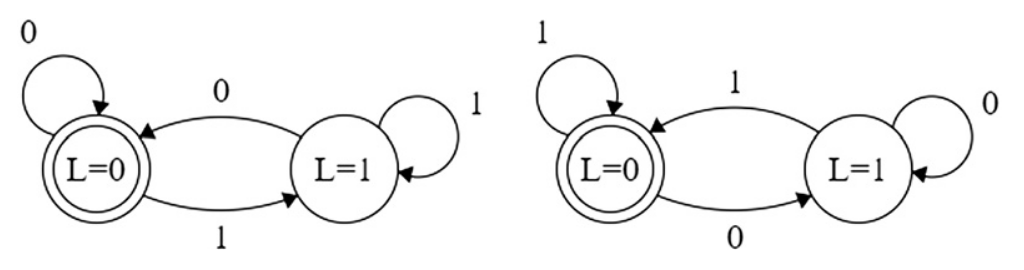
\includegraphics[width=3.1in]{img/dfsm.png}
        \caption{Deterministic finite state machine in which the start state is denoted by a double circle, the bit to be emitted is denoted by the label of each state, and the transitions dictated by the emitted bit of the interaction partner are denoted by the arrows. When supplied with the bits $\{1, 1, 0, 0, 1, 1\}$, the machine will emit $\{0, 0, 0, 1, 1, 0, 0\}$, first emitting the start state label and ending in the start state.}
        \label{dfsm}
    \end{center}
\end{figure}

Organisms in the game take the form of \textit{deterministic finite state machines} (DFSMs) as depicted in Figure \ref{dfsm}. Each state has either a 0 or 1 label, corresponding to the bit emitted at that state, and two transition links. The bit emitted by the other player determines which of the links to choose to transition to the next state. Due to the discrete nature of the machines, a loop eventually must occur in which both reach the same pair of states twice. The simulation ends once such a loop is detected, and the fitness for each player is determined by taking the average of all their scores in the loop.

Evolution begins with identical populations consisting of a single \textit{start state} with two links to itself. After each all-vs-all round of play, organisms are selected via \textit{fitness proportionate} selection and reproduce asexually. There is an equal probability that one of four mutations will occur:

\begin{enumerate}
    \item \textbf{Add state}: A new state is created, with two links created that each point to a state in the machine chosen uniformly at random (including the new state). The state does not yet have any links pointing to it, however, so this mutation will have a neutral effect on the phenotype until some other mutation connects it to the rest of the machine.
    \item  \textbf{Remove state}: A state is randomly selected with uniform probability for removal. Links from existing states that point to the removed state are redirected to the state pointed to by the corresponding link of the removed state if possible. If that link points to the removed state itself, the link is then connected to its origin. If a start state is selected for removal, then a new start state is selected from the remaining states with uniform probability. 
    \item \textbf{Change label}: A state is randomly selected and its bit is flipped.
    \item \textbf{Reassign link}: A link is chosen at random and reassigned to a randomly selected state.
\end{enumerate}

It was argued in \cite{moran2019} that ecosystems possessing only cooperative or competitive interactions tend to plateau in terms of complexity, there defined as the count of the number of states once a DFSM is pruned using \textit{Hopcroft's algorithm} \citep{Hopcroft1971AnNL}. Meanwhile, \textit{mixed} ecosystems were believed to hold the potential for \textit{unbounded growth}, determined as when the slope of the line of best fit to the mean complexity growth of a population exceeds that of a control or ``shadow'' ecosystem that lacks selection pressure. 

Various hypotheses were proposed in \cite{moran2019} to explain the behavior of the systems: that primarily cooperative species are more likely to exhibit growth; that \textit{convention chasing} may be responsible for cycles between competitive species, leading to \textit{evolutionary stable states}; and that clusters of competitive interactions appear to choke growth in larger configurations, leading to \textit{degenerate ecosystems} \citep{ficici1998, watson2002}. However, more comprehensive theoretical and statistical justification was left for future work, as the volume and apparent intricacy of the machines and their interactions made manual inspection and analysis intractable over evolutionary timescales. 

\subsection{The MODES Toolbox}
The \textit{MODES Toolbox} is a set of metrics and analytical techniques introduced in \cite{dolson2019} to better understand the open-ended potential of evolutionary systems in terms of change, novelty, complexity, and ecology. The toolbox produces results that support current intuitions and understanding of systems such as rugged NK landscapes and the Avida digital evolution platform \citep{Lenski2003TheEO, KAUFFMAN198711}. 

Before applying the metrics to evolutionary data, it is necessary to first screen out deleterious and neutral genotypes so that the focus is placed on truly adaptive lineages. The primary tool for doing so is the \textit{persistence filter}, a method with roots in an area of theoretical population genetics known as \textit{coalescence theory} \citep{Fu1999CoalescingIT}. The filter is used by identifying the \textit{persistent lineages} according to a sliding window of length $t$ generations. Coalescence theory predicts that in the absence of selective pressure, a single individual is expected to become the sole common ancestor of the entire population in a median time of $2N$ generations, where $N$ is the population size; this value typically becomes much smaller when selective pressure is present. At each generation $A - t$, each reproductive individual passes on to its offspring a unique identifier, which is passed on their offspring in turn if they are able to reproduce. This continues for $t$ generations until $A$ is reached, whereupon the identifiers are collected from members of the current population such that the persistent individuals from generation $A - t$ can be retrospectively identified.

This step alone dramatically reduce the volume of data for processing, at least by a factor of $N$, but there is more that can be done. It is recommended to identify the \textit{informative sites} of these persistent genotypes to prune noncoding genetic material. A simple means of doing so is the \textit{knockout} technique: For each site in the genotype, remove that site and observe the fitness effect for that individual in its original environment. If the fitness either remains the same or increases, this is evidence that the site is nonadaptive and can therefore be pruned. One downside of the technique is that interactions between sites may not be captured; more involved information-theoretical techniques may provide greater accuracy but are computationally infeasible for certain domains.

Once the persistent individuals and meaningful genotypic sites have been identified, the core MODES metrics can be applied at each generation interval $A$ given a window size of $t$:
\begin{enumerate}
    \item \textbf{Change}: A count of the number of unique persistent genotypes at generation $A$ that are different than those at generation $A - t$
    \item \textbf{Novelty}: A count of the number of persistent genotypes in generation $A$ that have not been seen at all in the intervals preceding it.
    \item \textbf{Complexity}: The greatest count of informative sites among all persistent genotypes at generation $A$
    \item \textbf{Ecology}: The Shannon entropy obtained from measuring the proportion of the persistent population occupied by each unique genotype at generation $A$. This metric provides an intuitive notion of diversity or evenness, as its value grows higher as a greater number of unique genotypes occupy more equal proportions of the population. 
\end{enumerate}

It was shown in \cite{dolson2019} that these metrics support common intuitions about multiple well-known evolutionary systems. For example, fitness-sharing and oscillating environments were shown to increase the change metric in NK landscapes. The novelty metric is shown to decrease over time in Avida as beneficial mutations are discovered and exploited; when novelty and change metrics appear similar, it implies that little cycling occurs over prior genotypes. In the Avida empty environment, the complexity metric spikes early on, then drops and remain constant, reflecting the fact that simpler solutions provide a greater fitness benefit in that environment. Meanwhile in the Logic 9 environment, a constant rise in complexity was observed as more difficult tasks were solved. 

\section{Experiments}
The motivation for employing the MODES Toolbox is threefold: (1), to test the hypotheses put forth in \cite{moran2019}, (2) as a form of data exploration to see what details might have been missed, and (3) to reduce a large, uninterpretable dataset to one more manageable for future data mining purposes. The codebase used for performing the experiments is available at \url{https://github.com/twillkens/coevo}.\footnote{We acknowledge computational support from the Brandeis HPCC, which is partially supported by the NSF through DMR-MRSEC 2011846 and OAC-1920147.}

Some design decisions were made to accommodate MODES within the linguistic prediction game environment. We strove to replicate the conditions of the original experiment as closely as possible, using a population size $N$ of fifty, fitness-proportionate selection, and uniform probability to select from each of the four types of mutation. The persistence window size $t$ is set to be the same size as the population, $N$: 50. For testing for uniqueness within the set of persistent components, we check if the two DFSMs are, when considered as graphs, \textit{isomorphic} according to an edge-preserving and label-preserving vertex bijection. (There are four possible state labels for the zero- and one-valued start states along with the zero- and one-valued inner states. The two directed edge values are zero and one.)

The complexity metric of \cite{moran2019} is defined as the count of the number of DFSM states following Hopcroft minimization. However, this only affects the structural properties of the graph and does not take fitness or phenotypic interaction into account. A preliminary application of the \textit{knockout} adaptive pruning method described in \cite{dolson2019} was found to have detrimental fitness effects in this domain on account of interactions between sites. A brute force solution that checks every combination of removals would be prohibitive given that the number of transitions increases combinatorially with the number of DFSM states and that some organisms comprise hundreds of states. To better identify meaningful sites in this particular representation, we employ a fitness-preserving heuristic that checks and prunes incrementally from the most recent to the oldest gene:

\begin{enumerate}
    \item Hopcroft's algorithm is applied to the original genotype to minimize the number of states.
    \item The resulting organism interacts with all of its partners in its generation, whose genotypes remain fixed. 
    \item All states in the subject that go untraversed in these interactions are pruned.
    \item Each remaining state is checked in order of genetic recency, with the most recently evolved state first. 
    \item The chosen state is removed and the resulting pruned individual again interacts with its fixed partners. 
    \item If the fitness of the new subject is greater than or equal to that of the original, the state is permanently removed; otherwise, it is replaced.
    \item Inspection continues with the next most recent state, and the process repeats until the oldest state has been checked.
    \item The resulting genotype is again minimized via Hopcroft's algorithm.
\end{enumerate}

Various pruning heuristics were tested in preliminary experiments, but the overall effect on the MODES metrics were similar between methods. A principled comparison of different pruning approaches, along with effects on the dynamics of the resulting organisms, could be a subject for future work.

\subsection{Two-Species Ecosystems}
We begin our analysis by focusing on ecosystem topologies with no more than two populations: the \textit{Control} ecosystem, which consists of two populations free to evolve without the influence of selective pressure; the \textit{Coop} ecosystem, in which both populations seek to match bits; and the \textit{Comp} ecosystem, where members of one population seek to match and the other to mismatch. Note that unless otherwise stated, the following figures depict the MODES metrics as applied to ecosystems as a whole and not to any particular populations within it.

\subsubsection{Statistical Methods}
MODES metrics are recorded for (1) persistent genotypes of all ecosystems following the use of Hopcroft's algorithm as in \cite{moran2019} and (2) persistent genotypes of ecosystems other than the Control using the incremental pruning heuristic described above. The KO labels denote these adaptive ``knockout'' groups. Statisical significance is assessed using Kruskal-Wallis tests with post-hoc Wilcoxon tests; Glass's $\Delta$ is used to quanfity effect size, where a value of 0.2 is generally considered a small effect, while a value of 0.8 is considered large.

\subsubsection{Change}

\begin{figure}[t]
    \begin{center}
        \includegraphics[width=3.1in]{img/2change.png}
        \caption{Change metric results for two-species ecosystems. Lines denote the mean taken over forty trials; shaded regions reflect a 95\% confidence interval.}
        \label{2change}
    \end{center}
\end{figure}

Change tracks the amount of turnover between genotypes at generations $A - t$ and $A$. If a genotype passes through the persistence filter at generation $A$, we look back to check whether the same genotype was present at $A - t$. If not, we count it as change.

In Figure \ref{2change}, we observe that the baseline Control group exhibits the highest rate of change relative to both the Coop group ($p < 0.0018$, Wilcoxon test; Glass's $\Delta = 0.85$) and Comp group ($p < 0.0065$, Wilcoxon test; Glass's $\Delta = 0.86$). This makes some intuitive sense given that a mutation operation is applied to every child and that Control lineages are free to explore the space of genotypes in an unrestrained manner. (Recall from \cite{moran2019} that as the size of our genotypes is bounded at one, mutations cannot produce negative genome sizes and thus average size of Control genotypes tends to increase over time due to genetic drift.) We notice that the Comp and Comp-KO groups exhibit the sharpest initial rise in change, likely reflecting the immediate pressure placed upon organisms by their counterparts. Notably, this change remains constant, implying that the inhabitants of this ecosystem cannot rest in one region of the genotype space for too long.

The Comp, and Comp-KO groups do not significantly differ, but the Coop-KO group exhibits far less change relative to the Control ($p < 0.0000001$, Wilcoxon test; Glass's $\Delta = 2.84$). We hypothesize that inhabitants of this ecosystem have little incentive to change their structure; in the absence of competitors, the most effective cooperator benefits from behaving as predictably as possible, and so their greatest threat is the change induced by the mutational velocity of the environment. Once adequate protective structures are in place, the rest of the genotype could be subject to random drift in a manner similar to the control. This suggests that our method is effective at pruning nonadaptive sites resulting from drift, and we thus hypothesize that Comp genotypes exhibit less nonadaptive ``bloat'' than those of Coop.

\subsubsection{Novelty}
\begin{figure}[t]
    \begin{center}
        \includegraphics[width=3.1in]{img/2novelty.png}
        \caption{Novelty metric results for two-species ecosystems. Lines denote the mean taken over forty trials; shaded regions reflect a 95\% confidence interval.}
        \label{2novelty}
    \end{center}
\end{figure}

The novelty results in Figure \ref{2novelty} first appear quite similar to the change results for all ecosystems involved. However, a closer look at the Comp-KO group shows novelty gradually decreasing over time. Comparing the slopes obtained through least squares regression over the means of the last 25,000 generations of the Comp-KO change ($X = -0.000016$, $p < 0.722$) and novelty ($X = -0.00022$, $p < 0.0001$) metrics, we find that novelty has a comparatively significant downward slope. It is proposed in \cite{dolson2019} that a constant change metric with a decreasing novelty score is evidence of cycling over genotype space. This tracks with the hypothesis in \cite{moran2019} that competitive species may fall prey to \textit{convention chasing} cycles resulting in an evolutionary stable state \cite{ficici1998}. This trend is subtle, which suggests that there is ample room for exploration within the space; further long-term experimentation could show whether novelty values in fact converge to zero.

The positive novelty slopes of Control (X = $0.0009$, $p < 0.00001$) and Coop (X = $0.0003$, $p < 0.00001$) support the intuition that as the genotypes grow larger on account of drift, the space of possible novelties increases. We note also that the final novelty metric of the Coop-KO group is extremely low relative to Control ($p < 0.0000001$, Wilcoxon test; Glass's $\Delta = 4.13$), matching the intuition that small, stable genotypes are more likely to retread old ground. This gives some evidence that the persistence filter successfully screens out duplicates.

\subsubsection{Complexity}
\begin{figure}[t]
    \begin{center}
        \includegraphics[width=3.1in]{img/2complexity.png}
        \caption{Complexity metric results for the two-species ecosystems. Lines denote the mean taken over forty trials; shaded regions reflect a 95\% confidence interval.}
        \label{2complexity}
    \end{center}
\end{figure}

The complexity curves of the Hopcroft-pruned Control, Comp, and Coop groups in Figure \ref{2complexity} mirror those in \cite{moran2019}, indicating that our use of the toolbox does not greatly distort the original results. We see the Control and Coop ecosystems grow over time on account of the fact that size of the organism is bounded above zero; while Coop appears to trend higher, the two groups do not significantly differ in the final generation ($p < 0.69$, Wilcoxon test; Glass's $\Delta = 0.07$). We likewise see the Comp group rise early before leveling out below the control ($p < 0.000001$, Wilcoxon test; Glass's $\Delta = 3.64$). Most salient is the observation that Coop-KO complexity is dramatically lower than that of Control ($p < 0.0000001$, Wilcoxon test; Glass's $\Delta = 26.5$). The Comp-KO group also is significantly reduced in complexity ($p < 0.0000001$, Wilcoxon test; Glass's $\Delta = 18.7$), but with less effect than Coop-KO, inverting the relationship between the unaltered groups.

This makes sense when we consider the logical consequences of performing knockout on the Coop organisms. Individuals are incentivized to enter a loop as soon as possible in order to maximize fitness; thus, pruning away neutral or deleterious states could end up removing large portions of the machine.


\subsubsection{Episode Length}
\begin{figure}[t]
    \begin{center}
        \includegraphics[width=3.1in]{img/2eplen.png}
        \caption{Average episode lengths among the two-species ecosystems. Lines denote the mean taken over forty trials; shaded regions reflect a 95\% confidence interval.}
        \label{2eplen}
    \end{center}
\end{figure}

To support this intuition, Figure \ref{2eplen} shows the episode lengths for the two-species ecosystems, defined as the sum of the length of the transient period and the length of the loop. The Coop ($p < 0.000001$, Wilcoxon test; Glass's $\Delta = 2.3$) and Coop-KO ($p < 0.0000001$, Wilcoxon test; Glass's $\Delta = 3.9$) groups have the shortest episodes relative to the control, with the majority of their interactions lasting fewer than five timesteps. If by the end of a run a machine has over seventy states but uses only a fraction in practice, we can expect that the great majority yield neutral results and could be safely pruned.

The Comp group ends the run with longer episodes than Control ($p < 0.000001$, Wilcoxon test; Glass's $\Delta = -1.34$), but the slope of Comp ($X = -0.0003$, $p < 0.11$) plateaus in contrast to the Control's slow rise ($X = 0.005$, $p < 0000001$). This may indicate strategy cycling among Comp species, while the Control interactions may grow longer over evolutionary time in the absence of selection as it takes longer on average for enter a loop. 

\begin{figure}[t]
    \begin{center}
        \includegraphics[width=3.1in]{img/2fitness.png}
        \caption{Fitness metric among the two-species ecosystems. Lines denote the mean taken over forty trials; shaded regions reflect a 95\% confidence interval.}
        \label{2fitness}
    \end{center}
\end{figure}

It must be noted that the typical Comp-KO episode length is shorter relative to Comp ($p < 0.000001$, Wilcoxon test; Glass's $\Delta = 1.24$), indicating that removing maladaptive sites yields different phenotypic behavior. We can verify the optimization effect of adaptive pruning in Figure \ref{2fitness}, where we note that the Comp group is less fit than Comp-KO ($p < 0.0000001$, Wilcoxon test; Glass's $\Delta = -0.85$).

\begin{figure}[t]
    \begin{center}
        \includegraphics[width=3.1in]{img/2coverage.png}
        \caption{Coverage metric among the two-species ecosystems. Lines denote the mean taken over forty trials; shaded regions reflect a 95\% confidence interval.}
        \label{2coverage}
    \end{center}
\end{figure}
We propose the \textit{coverage} statistic to probe the conjecture that the majority of Coop states go unused even following Hopcroft minimization. This is defined as the proportion of states traversed at least once during the course of an episode relative to the size of the organism, averaged over all interactions. We observe in Figure \ref{2coverage} that the KO groups have very high rates of coverage, indicating that adaptive pruning is succeeding in its aim. The Coop group has the lowest rate of coverage relative to Control ($p < 0.01$, Wilcoxon test; Glass's $\Delta = 0.61$), further suggesting that members of the Coop group are more likely to have unused states. 

\subsubsection{Ecology}
\begin{figure}[t]
    \begin{center}
        \includegraphics[width=3.1in]{img/2ecology.png}
        \caption{Ecology metric among the two-species ecosystems. Lines denote the mean taken over forty trials; shaded regions reflect a 95\% confidence interval.}
        \label{2ecology}
    \end{center}
\end{figure}

We observe in Figure \ref{2ecology} that the Control group supports the most diverse ecology, suggesting that the absence of selection allows for a broader range of genotypes to coexist. We notice that the adaptive pruning only slightly affects the ecology metric of the Comp-KO group ($p < 0.03$, Wilcoxon test; Glass's $\Delta = 0.21$), while greatly reducing the Coop-KO group ($p < 0.000001$, Wilcoxon test; Glass's $\Delta = 1.69$). This may reflect the efficacy of interactions between identical genotypes among species in the Coop ecosystem.

\begin{figure}[t]
    \begin{center}
        \includegraphics[width=3.1in]{img/3change.png}
        \caption{Change metric among the three-species ecosystems. Lines denote the mean taken over forty trials; shaded regions reflect a 95\% confidence interval.}
        \label{3change}
    \end{center}
\end{figure}

\begin{figure}[t]
    \begin{center}
        \includegraphics[width=3.1in]{img/3novelty.png}
        \caption{Novelty metric among the three-species ecosystems. Lines denote the mean taken over forty trials; shaded regions reflect a 95\% confidence interval.}
        \label{3novelty}
    \end{center}
\end{figure}

\begin{figure}[t]
    \begin{center}
        \includegraphics[width=3.1in]{img/3complexity.png}
        \caption{Complexity metric among three-species ecosystems. Lines denote the mean taken over forty trials; shaded regions reflect a 95\% confidence interval.}
        \label{3complexity}
    \end{center}
\end{figure}

\begin{figure}[t]
    \begin{center}
        \includegraphics[width=3.1in]{img/3ecology}
        \caption{Ecology metric among the three-species ecosystems. Lines denote the mean taken over forty trials; shaded regions reflect a 95\% confidence interval.}
        \label{3ecology}
    \end{center}
\end{figure}

\subsection{Three-Species Ecosystems}
In \cite{moran2019}, the hypothesis is proposed that for ecosystems with three or more species, purely competitive and cooperative interaction types lead to stagnation, while mixed ecosystems hold the potential for unbounded complexity growth. The data obtained using the MODES Toolbox suggests that, for at least one ecosystem, the observed complexity growth is largely nonadaptive.

In the original work, the cooperative species of the 3-Mixed ecosystem was the only one to exhibit unbounded growth, while the competitive and mixed species plateaued. This was hypothesized to result from long-term adaptation by the cooperator to accommodate rapid cycling between its partner and the partner's competitor.

Here we discover some intriguing differences. First we observe in Figure \ref{3change} a lower overall effect size compared to the two-species variety; the 3-Comp ecosystem fails to reject the null hypothesis of no difference from 3-Control ($p < 0.11$, Wilcoxon test; Glass's $\Delta = 0.43$). While the 3-Mixed-KO ecosystem appears to exhibit the least amount of change on average, at the final generation the result is actually not significantly different than 3-Control ($p < 0.28$, Wilcoxon test; Glass's $\Delta = 0.33$); tests performed at previous generations do find a difference, as in generation 49,500 ($p < 0.0027$, Wilcoxon test; Glass's $\Delta = 0.86$), so more trials and generations may be needed for conclusive results. Visually it appears that the 3-Mixed-KO group exhibits less change than the 3-Comp group; if borne out statistically, this would lend some support to Moran's thesis, as slower-evolving cooperative species might moderate overall evolutionary activity compared with 3-Comp, in which all species are trying to outpace their rivals. Similar trends are observed in the novelty plot of Figure \ref{3novelty} and ecology plot of Figure \ref{3ecology}.

Finally, from \cite{moran2019} we would also expect that the 3-Mixed ecosystem to exhibit the greatest complexity growth in comparison with the 3-Comp ecosystem, which was regarded as stagnant. However, adaptive pruning dramatically reduces the complexity of the 3-Mixed-KO group relative to 3-Mixed ($p < 0.0000001$, Wilcoxon test; Glass's $\Delta = 13.11$). This result suggests that observed complexity growth of the 3-Mixed ecosystem requires qualification and further investigation. One conjecture is that the complexity growth, which clearly exceeds 3-Control in the 3-Mixed case ($p < 0.0001$, Wilcoxon test; Glass's $\Delta = -1.27$), is more akin to the spandrels of \cite{Gould1979TheSO} than the product of adaptive evolution, but the precise mechanism is still unclear.  

\begin{figure}[t]
    \begin{center}
        \includegraphics[width=3.1in]{img/3eplen}
        \caption{Episode length metric among the three-species ecosystems. Lines denote the mean taken over forty trials; shaded regions reflect a 95\% confidence interval.}
        \label{3eplen}
    \end{center}
\end{figure}

\begin{figure}[t]
    \begin{center}
        \includegraphics[width=3.1in]{img/3coverage.png}
        \caption{Coverage metric among the three-species ecosystems. Lines denote the mean taken over forty trials; shaded regions reflect a 95\% confidence interval.}
        \label{3coverage}
    \end{center}
\end{figure}

To support this notion, we observe in Figure \ref{3eplen} that the 3-Comp ecosystem clearly exceeds 3-Mixed in terms of episode length, which we would not expect if the greater genotypic complexity of 3-Mixed were being utilized. We also note that in Figure \ref{3coverage}, the symbiote species of 3-Mixed exhibits a much lower rate of coverage than 3-Control ($p < 0.00001$, Wilcoxon test; Glass's $\Delta = 1.13$).

\section{Conclusion and Future Work}
Application of the MODES Toolbox to the linguistic prediction game has proven fruitful, providing a variety of interesting observations and raising new questions. Various intuitions about the behavior of two-species ecosystems have been given statistical support, including the hypothesis that competitive species are prone to cycling behavior leading to evolutionary stable states. Adaptive pruning is shown to significantly reduce genotypic bloat in the Coop ecosystem, even after the application of structural pruning, allowing a better understanding of the distinction between adaptive and nonadaptive complexity in this domain. 

More trials and longer simulations are needed for conclusive interpretations of the three-species ecosystems, but one unambiguous result is that the complexity observed in the 3-Mixed ecosystem appears largely nonadaptive. This is supported by supplementary metrics such as episode length and DFSM state coverage, which raises the question of precisely how the observed growth in the Hopcroft group manages to exceed the control. We conjecture that cycling dynamics between the competitive species may necessitate periods of growth close to the start state in the cooperative group, while the rest of the genotype is free to grow on account of drift. Experiments are needed to test this possibility as well as gauge the viability of alternative explanations.

Additional future work could involve the application of MODES to the \textit{collision game} of \cite{willkens2022}, which employs a recurrent neural network organism representation in an analogous domain. In that work, an incremental pruning experiment over a single generation was indicative of adaptive growth, but a more comprehensive and principled approach such as MODES might produce a more conclusive interpretation. Combining MODES with the visualization techniques of \cite{dolson2020}, adapted for particular domains and organism representations, could provide a richer picture of the open-ended dynamics of a variety of coevolutionary games, including those yet to be discovered.


% \setcounter{figure}{4}

% \begin{figure*}
%     \begin{center}
%       \includegraphics[width=0.9\textwidth]{graphs.png}
%       \caption{Average population complexity over all trials in terms of number of expressed network connections.}
%       \label{fig:allgraphs}
%     \end{center}
% \end{figure*}

%\clearpage

%\FloatBarrier

\footnotesize
\bibliographystyle{apalike}
\bibliography{modes.bib} % replace by the name of your .bib file


\end{document}
